\documentclass[12pt]{article}
\usepackage[utf8]{inputenc}
\usepackage[greek,english]{babel}
\usepackage{alphabeta}
\usepackage{fancyhdr}
\usepackage{listings}
\usepackage{mathtools}
\usepackage{xcolor}
\usepackage{float}
\usepackage{siunitx}
\usepackage[margin=0.5in]{geometry}
\usepackage[backend=bibtex]{biblatex}
\addbibresource{cit.bib}

\title{Εργαστήριο Μικροηλεκτρονικής -- Εργασία 1}
\author{Χρήστος Μαργιώλης -- 19390133}
\date{Απρίλιος 2022}

\begin{document}

\begin{titlepage}
        \maketitle
        \begin{figure}[t!]
        \begin{center}
        
\includegraphics[scale=0.3]{./res/uniwalogo.png} \\
        \Large
        \textbf{Πανεπιστήμιο Δυτικής Αττικής} \\
        \large
        Τμήμα Μηχανικών Πληροφορικής και Ηλεκτρονικών Υπολογιστών
        \end{center}
        \end{figure}
\end{titlepage}

\renewcommand{\contentsname}{Περιεχόμενα}
\tableofcontents
\pagebreak

\section{Θεωρητικό μέρος}

Η εργασία αυτή έχει ως θέμα την υλοποίηση και μελέτη τελεστικών ενισχυτών.
Τελεστικός ενισχυτής είναι ένα κύκλωμα το οποίο, πέρα από το ότι έχει
ενισχυτική ικανότητα, μπορεί να εκτελέσει και μαθηματικές πράξεις (τελεστές),
όπως πρόσθεση, αφαίρεση, πολλαπλασιαμό, διαίρεση, παραγώγηση και ολοκλήρωση.
'Ενα άλλο χαρακτηριστικό των τελεστικών ενισχυτών είναι η τεράστια ενίσχυση που
προσφέρουν, ακόμα και με πολύ μικρές διαφορές δυναμικού.

Παρόλα αυτά, η τόσο μεγάλη ενισχυτική ικανότητα που παρέχουνε, δεν είναι
ιδιαίτερα χρήσιμη, οπότε χρησιμοποιούμε μεγάλες αντιστάσεις ώστε να
περιορίσουμε το κέρδος (gain) του ενισχυτή.

Μερικές από τις θεμελιώδεις συνδεσμολογίες τελεστικών ενισχυτών είναι οι
παρακάτω:
\begin{itemize}
	\item Συγκριτής τάσης (voltage comparator).
	\item Αναστρέφων τελεστικός ενισχυτής (inverting operational
		amplifier).
	\item Μη-αναστρέφων τελεστικός ενισχυτής (non-inverting operational
		amplifier).
	\item Απομονωτής (buffer).
\end{itemize}

Ο συγκριτής τάσης δέχεται μία είσοδο και μία τάση αναφοράς (reference voltage),
και έχει 2 πιθανές εξόδους που θα μπορούσαμε να παρομοιάσουμε με το λογικό 0
και 1, ή με την δομή if-else. Πιο συγκεκριμένα, αν η τάση εισόδου είναι
μικρότερη της τάσης αναφοράς, τότε η έξοδος είναι η θετική τάση $V_{cc}$,
αλλιώς στην αντίθετη περίπτωση, η έξοδος είναι η αρνητική τάση $V_{ee}$.
Δηλαδή:
\[
	V_o = 
	\left\{
		\begin{array}{ll}
		V_{cc} & V_{in} < V_{ref} \\
		V_{ee} & V_{in} > V_{ref} \\
	\end{array}
	\right.
\]

Ο αναστρέφων τελεστικός ενισχυτής αναστρέφει το σήμα εισόδου και έχει διαφορά
φάσης \SI{180}{\degree}. Η αναστροφή αυτή επιτυγχάνεται με την σύνδεση του
σήματος εισόδου στον αρνητικό ακροδέκτη $V_n$ του ενισχυτή.

Ο μη-αναστρέφων ενισχυτής έχει αντιστραμένες τις εισόδους από τον αναστρέφοντα
ενισχυτή, και η αντίσταση εισόδου είναι γειωμένη. Το σήμα εξόδου του είναι σε
φάση με το σήμα εισόδου, και πρέπει οπωσδήποτε να έχει κέρδος μεγαλύτερο του 1.

Ο buffer έχει πολύ μεγάλη αντίσταση εισόδου και μοναδιαίο κέρδος, οπότε είναι
ιδανικός για σύνδεση κυκλωμάτων χωρίς να υπάρχει απώλεια σήματος. Στην υλοποίηση
του είναι ένας μη-αναστρέφων τελεστικός ενισχυτής, με την διαφορά ότι λείπει η
feedback αντίσταση.

\section{Αναζήτηση βιβλιογραφίας}

Η βιβλιογραφία που χρησιμοποιήθηκε είναι δύο ακαδημαϊκά άρθρα, ένα από το MIT
\cite{mit} και ένα από το Πολυτεχνείο της Καλοφόρνια \cite{cpp}. Περισσότερες
πληροφορίες βρίσκονται στο τέλος της εργασίας.

\section{Υλοποίηση της εργασίας}

Για την υλοποίηση της εργασίας χρησιμοποιήθηκαν τα παρακάτω εργαλεία:
\begin{itemize}
	\item Tina-TI για την συνδεσμολογία και τις μετρήσεις του κυκλώματος.
	\item Tinkercad για την υλοποίηση του κυκλώματος σε breadboard.
	\item Latex για την συγγραφή της εργασίας.
\end{itemize}

\section{Συνδεσμολόγηση κυκλώματος}

\begin{itemize}
	\item Συνδεσμολογήστε το παρακάτω κύκλωμα με
		$R_1 = R_2 = \SI{100}{\kilo\ohm}$ και
		$V_1 = \SI{15}{\volt}$,
		$V_2 = \SI{-15}{\volt}$.
\end{itemize}

Η χρήση αντιστάσεων στο παρακάτω κύκλωμα, καθώς και η σύνδεση του θετικού
ακροδέκτη του ενισχυτή στην γη, δείχνει ότι το κύκλωμα πρόκειται για έναν
αναστρέφοντα τελεστικό ενισχυτή.

\begin{figure}[H]
	\centering
	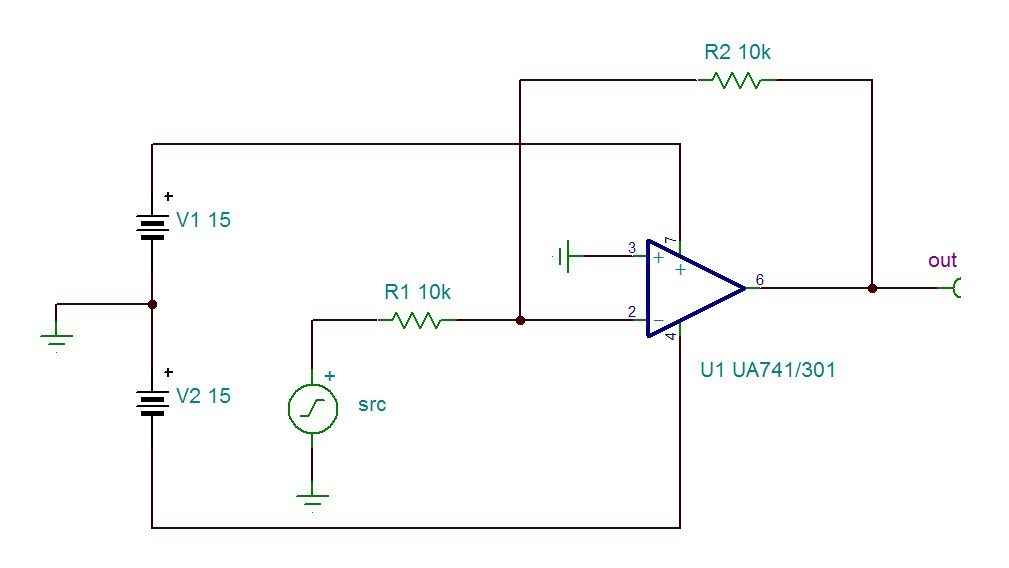
\includegraphics[width=\linewidth]{./res/schem.jpg}
	\caption{Αναστρέφων τελεστικός ενισχυτής}
\end{figure}

\section{Εφαρμογή σήματος}

\begin{itemize}
	\item Εφαρμόστε ημιτονικό σήμα $\SI{1}{\kilo\hertz}/1V_{pp}$ στην είσοδο.
	\begin{itemize}
		\item Αναπαραστήσετε σε γράφημα την έξοδο του κυκλώματος ως
			προς την είσοδο.
		\item Υπολογίστε το θεωρητικό και πρακτικό κέρδος του ενισχυτή,
			στη συνέχεια συγκρίνατε τα δύο κέρδη. Υπάρχουν
			διαφορές; Πού οφείλονται;
		\item Μετρήστε την διαφορά φάσης που παρατηρείται μεταξύ
			εισόδου και εξόδου.
	\end{itemize}
\end{itemize}

\subsection{Γράφημα εξόδου ως προς είσοδο}

Με την αναπαράσταση της εξόδου του κυκλώματος ως προς την είσοδο, συμπεραίνουμε
ότι πράγματι το κύκλωμα είναι ένας αναστρέφων τελεστικός ενισχυτής, εφόσον το
σήμα εξόδου είναι $\SI{180}{\degree}$ εκτός φάσης.

\begin{figure}[H]
	\centering
	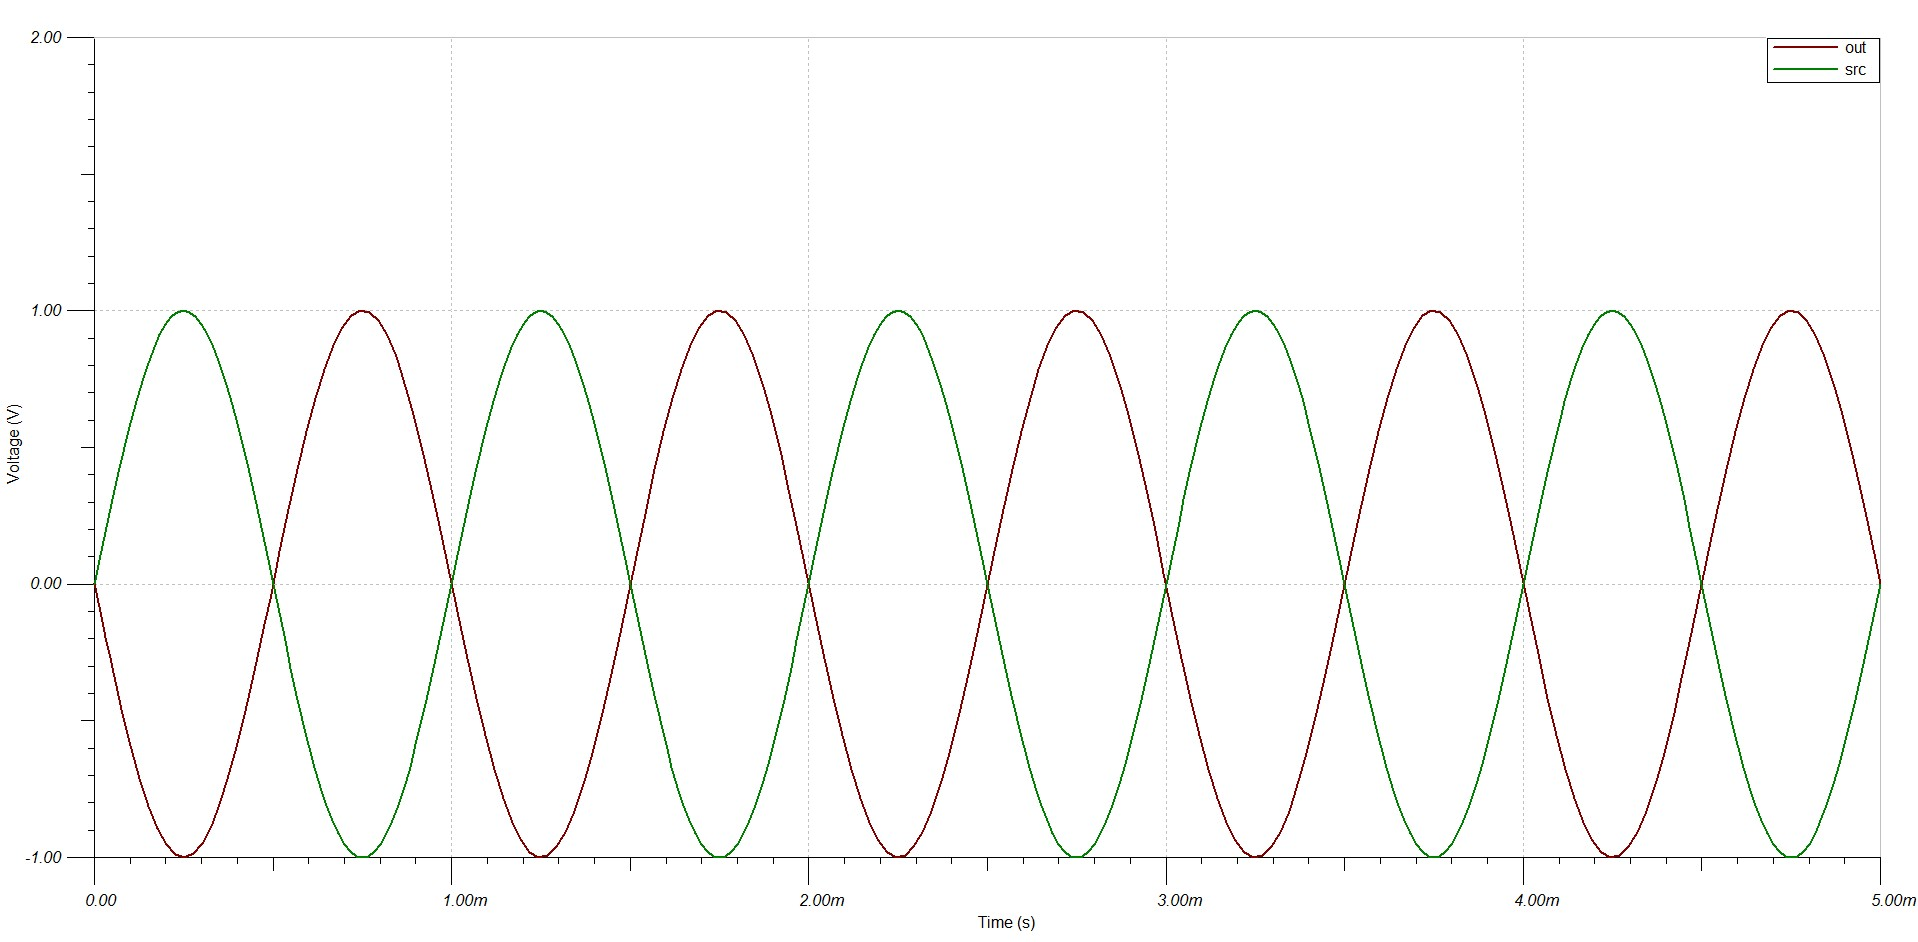
\includegraphics[width=\linewidth]{./res/out1.jpg}
	\caption{Καμπύλες στο ίδιο γράφημα}
\end{figure}

\begin{figure}[H]
	\centering
	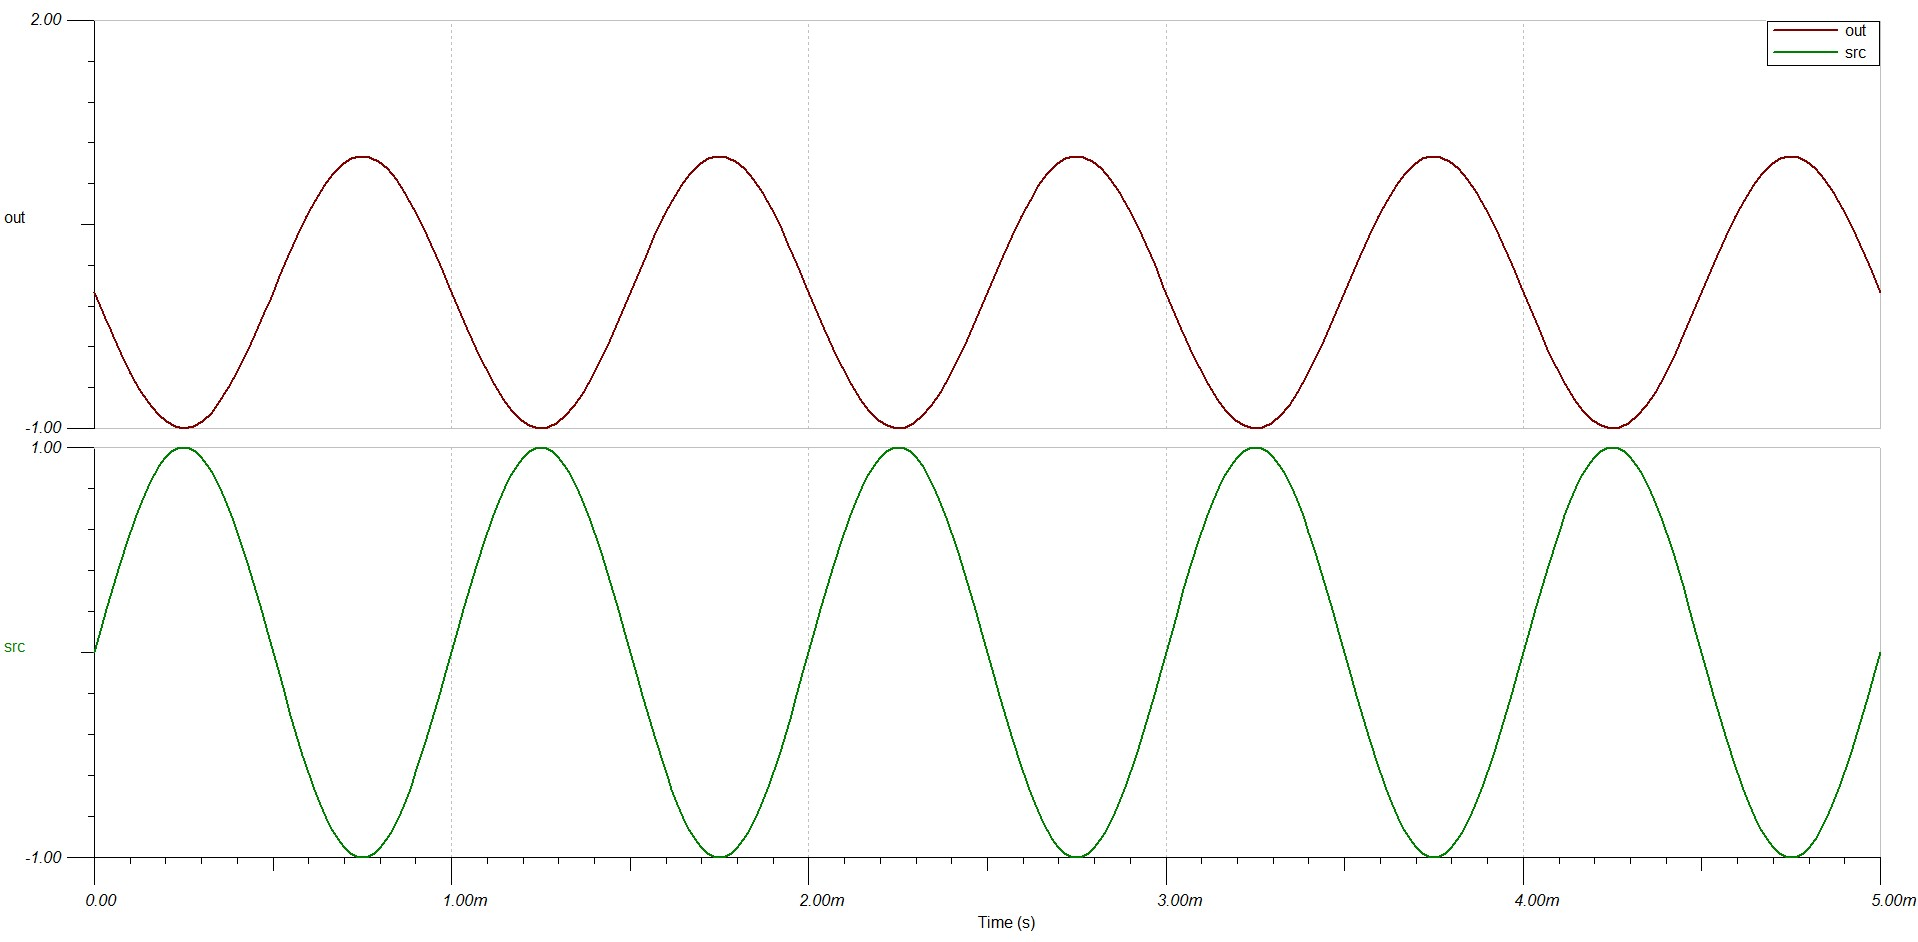
\includegraphics[width=\linewidth]{./res/out2.jpg}
	\caption{Καμπύλες σε ξεχωριστό γράφημα}
\end{figure}

\subsection{Θεωρητικό και πρακτικό κέρδος}

Το θεωρητικό κέρδος του αναστρέφοντα ενισχυτή υπολογίζεται από τον τύπο:
\[A_v = -\frac{R_2}{R_1}\]
Οπότε, έχουμε ότι:
\[
	A_v = -\frac{R_2}{R_1} \Rightarrow
	A_v = -\frac{\SI{10}{\kilo\ohm}}{\SI{10}{\kilo\ohm}} \Rightarrow
	A_v = -1
\]
Μετατρέπουμε το κέρδος σε \SI{}{\decibel}:
\[
	A_v(\SI{}{\decibel}) = 20\log_{10}\lvert A_v \lvert \Rightarrow
	A_v(\SI{}{\decibel}) = 20\log_{10}\lvert -1 \lvert \Rightarrow
	A_v(\SI{}{\decibel}) = \SI{0}{\decibel}
\]

Το πρακτικό κέρδος, με βάση την παρακάτω μέτρηση, είναι
\SI{0.000733}{\decibel}. Παρατηρούμε ότι το θεωρητικό και πρακτικό κέρδος δεν
απέχουν πολύ -- θα μπορούσαμε να υποθέσουμε ότι είναι και ίδια. Ο λόγος που δεν
μπορεί το πρακτικό κέρδος να είναι 100\% ίδιο με το θεωρητικό, οφείλεται στο
γεγονός ότι στην πραγματικότητα, τα υλικά των κυκλωμάτων (αντιστάσεις,
πυκνωτές, κλπ), επηρεάζονται από φυσικούς παράγοντες (π.χ θερμότητα) και έτσι
δεν λειτουργούνε με βάση τις ιδανικές συνθήκες με τις οποίες λειτουργούν οι
μαθηματικοί τύποι.

Παρατηρούμε επίσης ότι μετά από μία συγκεκριμένη συχνότητα, το κέρδος αρχίζει
και πέφτει. Αυτό οφείλεται στο ότι η συχνότητα του σήματος εισόδου ξεπερνάει
την ταχύτητα με την οποία ο ενισχυτής μπορεί να επεξεργαστεί το σήμα.

\begin{figure}[H]
	\centering
	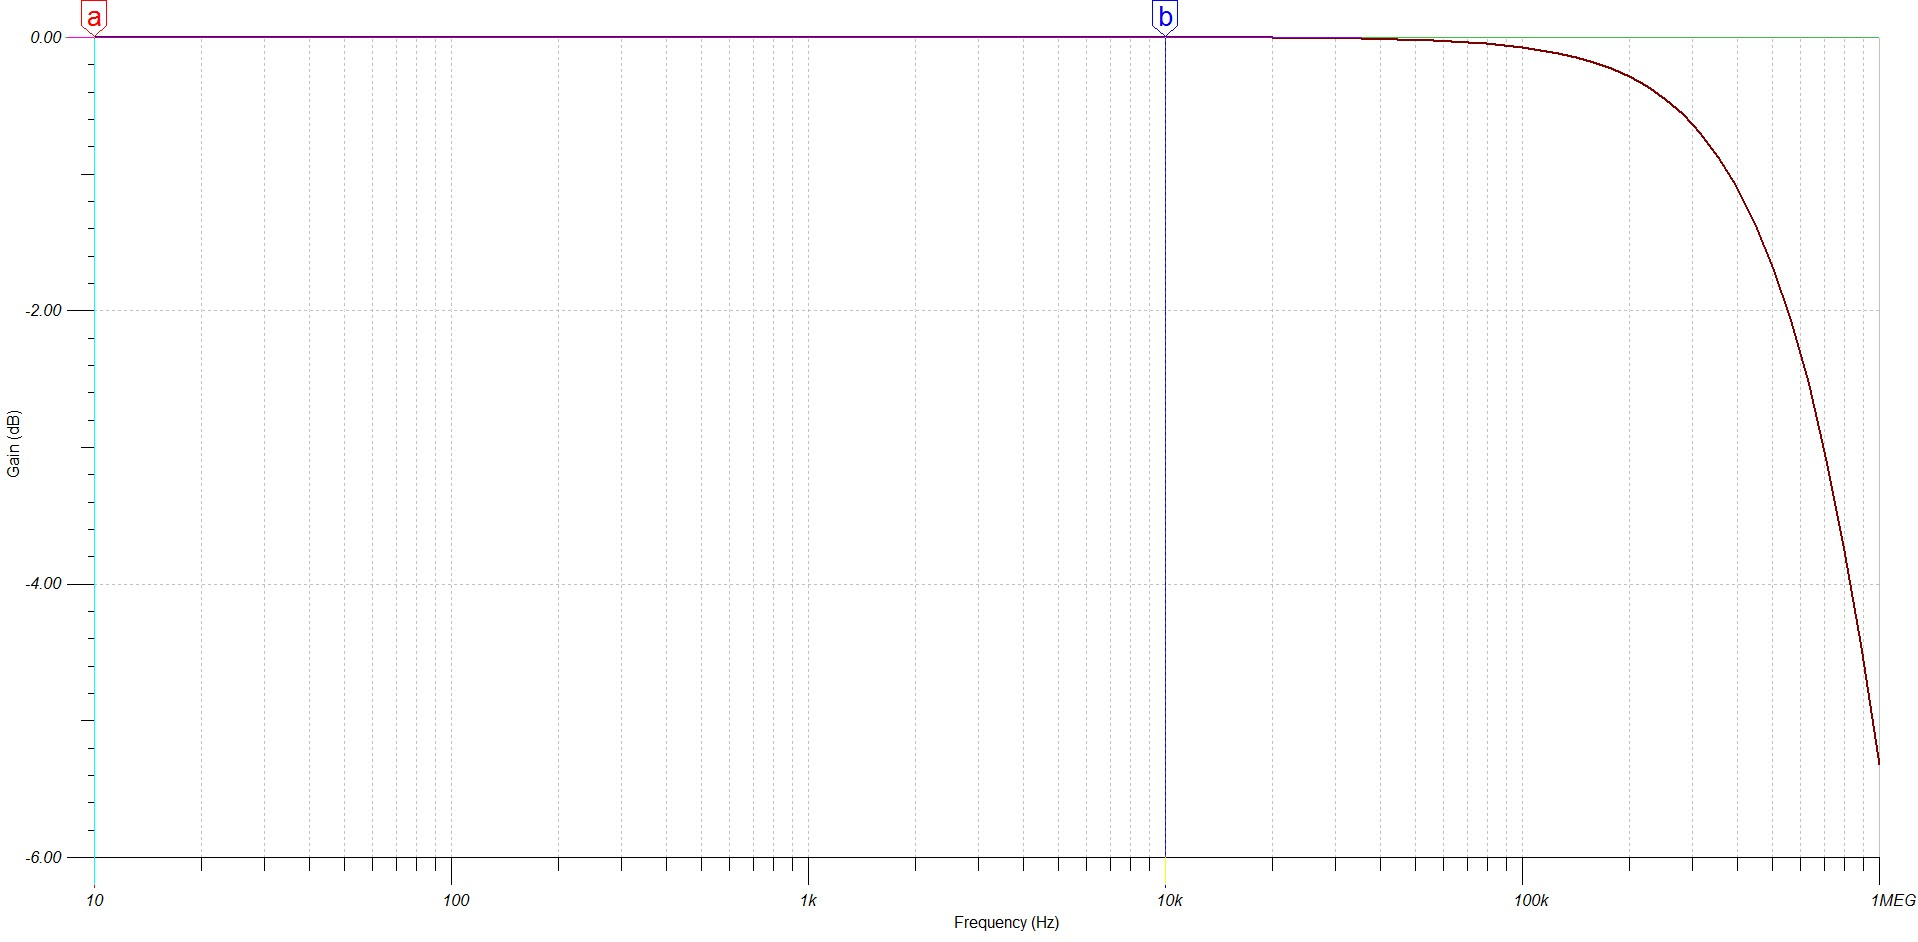
\includegraphics[width=\linewidth]{./res/gain.jpg}
	\caption{Γράφημα πρακτικού κέρδους}
\end{figure}
\begin{figure}[H]
	\centering
	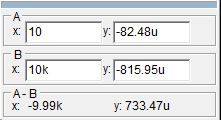
\includegraphics{./res/gaincalc.jpg}
	\caption{Υπολογισμός πρακτικού κέρδους}
\end{figure}

\subsection{Διαφορά φάσης}

Με βάση την παρακάτω μέτρηση, η διαφορά φάσης είναι περίπου \SI{\pi}{\radian}
(\SI{180}{\degree}), μέχρι που αρχίζει και πέφτει λογαριθμικά. Δηλαδή, το σήμα
εισόδου βρίσκεται σε αντίθετη φάση με το σήμα εξόδου. 'Οπως και με την μέτρηση
του πρακτικού κέρδους, έτσι και η διαφορά φάσης δεν μπορεί να αντιστοιχεί
ακριβώς στα θεωρητικά αποτελέσματα, αλλά είναι πάρα πολύ κοντά.

\begin{figure}[H]
	\centering
	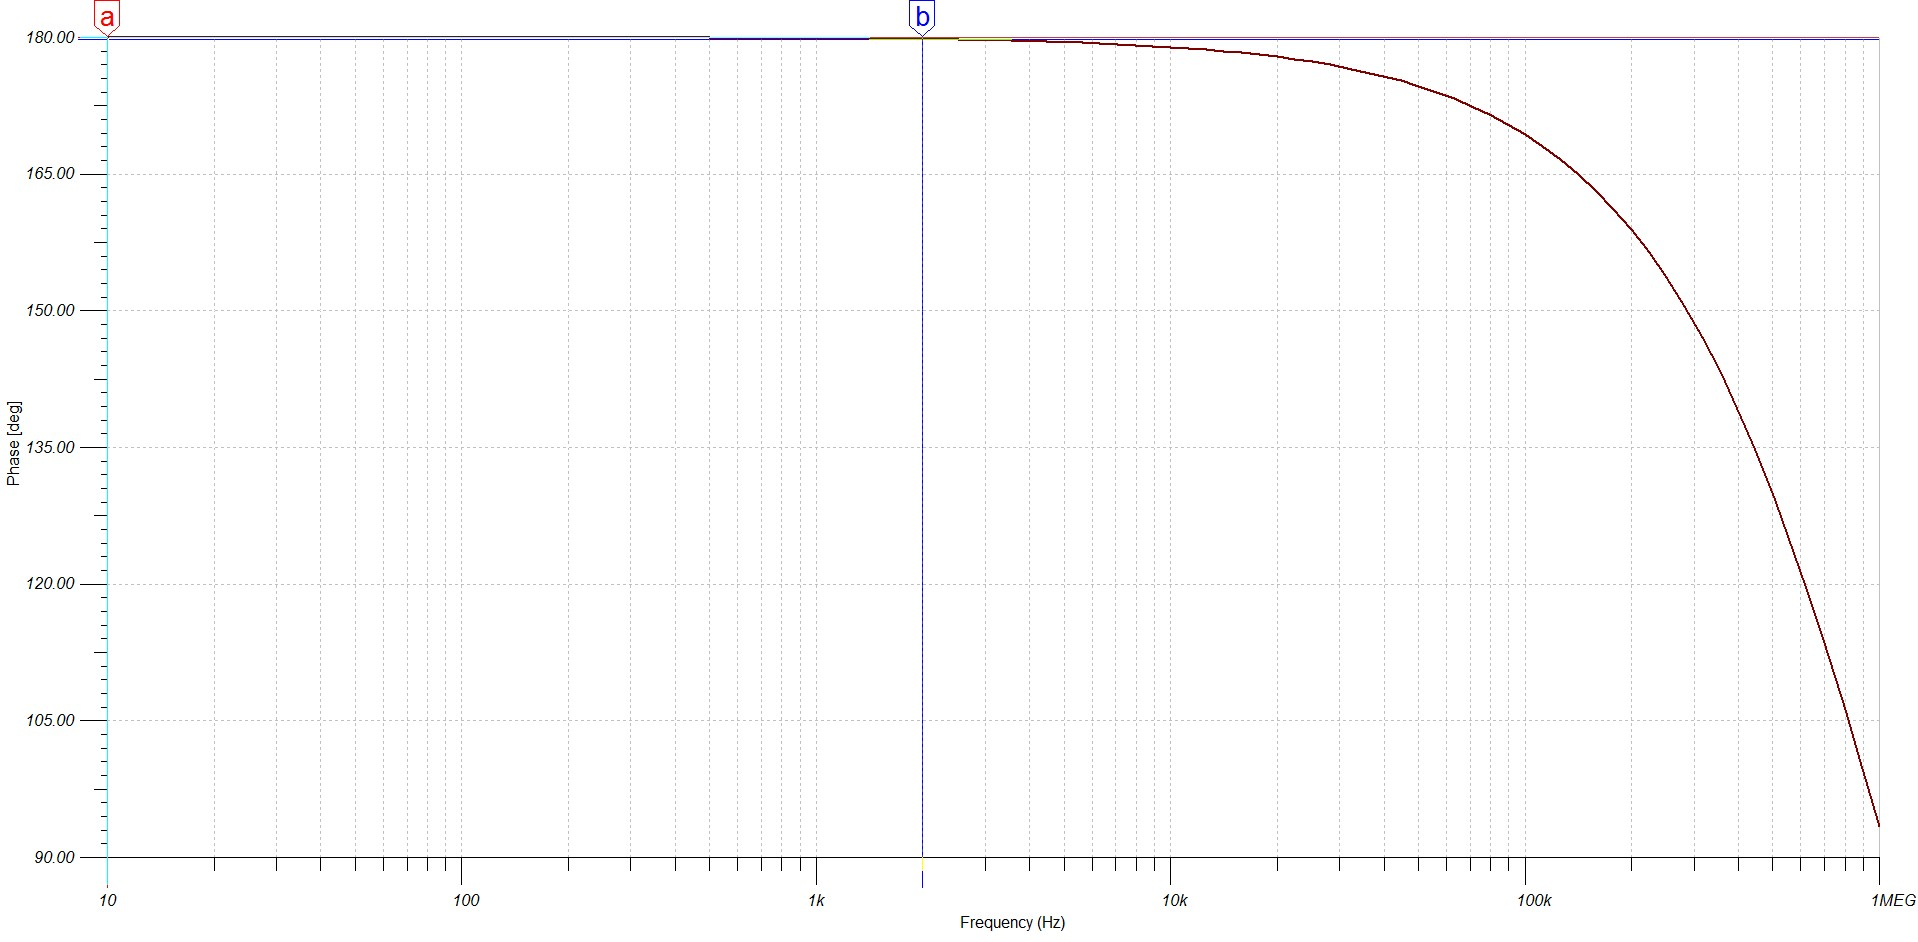
\includegraphics[width=\linewidth]{./res/phase.jpg}
	\caption{Γράφημα φάσης}
\end{figure}
\begin{figure}[H]
	\centering
	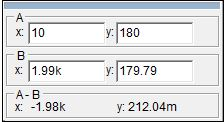
\includegraphics{./res/phasecalc.jpg}
	\caption{Υπολογισμός διαφοράς φάσης}
\end{figure}

\section{Αύξηση συχνότητας}

\begin{itemize}
	\item Διατηρώντας το πλάτος του σήματος εισόδου σταθερό αυξήστε την
		συχνότητα εισόδου σύμφωνα με τον παρακάτω πίνακα. Τι
		παρατηρείτε; Πού οφείλεται;
\end{itemize}

Από τον παρακάτω πίνακα, παρατηρούμε ότι ασχέτως του πόσο θα αυξηθεί η
συχνότητα του σήματος εισόδου, το κέρδος είναι ίδιο. Αυτό οφείλεται στο ότι ο
ενισχυτής έχει \SI{0}{\decibel} θεωρητικό (και 0.000733 πρακτικό) κέρδος, οπότε
εφόσον ο ενισχύτης δεν έχει κέρδος, τότε όσο και να αυξήσουμε την συχνότητα, θα
εξακολουθούμε να μην έχουμε κέρδος, αν δεν αλλάξουμε και το πλάτος του σήματος
εισόδου.

\begin{center}
\begin{tabular}{|l|l|}
	\hline
	$F(\SI{}{\hertz})$ & $A(\SI{}{\decibel})$ \\
	\hline
	$\SI{1}{\kilo\hertz}$ & \SI{0}{\decibel} \\
	\hline
	$\SI{10}{\kilo\hertz}$ & \SI{0}{\decibel} \\
	\hline
	$\SI{50}{\kilo\hertz}$ & \SI{0}{\decibel} \\
	\hline
	$\SI{100}{\kilo\hertz}$ & \SI{0}{\decibel} \\
	\hline
	$\SI{500}{\kilo\hertz}$ & \SI{0}{\decibel} \\
	\hline
	$\SI{1}{\mega\hertz}$ & \SI{0}{\decibel} \\
	\hline
	$\SI{1.5}{\mega\hertz}$ & \SI{0}{\decibel} \\
	\hline
	$\SI{2}{\mega\hertz}$ & \SI{0}{\decibel} \\
	\hline
\end{tabular}
\end{center}

\section{Υλοποίηση σε breadboard}

\begin{itemize}
	\item Παρουσιάστε το κύκλωμά σας υλοποιημένο σε breadboard μέσω
		της εφαρμογής Tinkercad.
\end{itemize}

\begin{figure}[H]
	\centering
	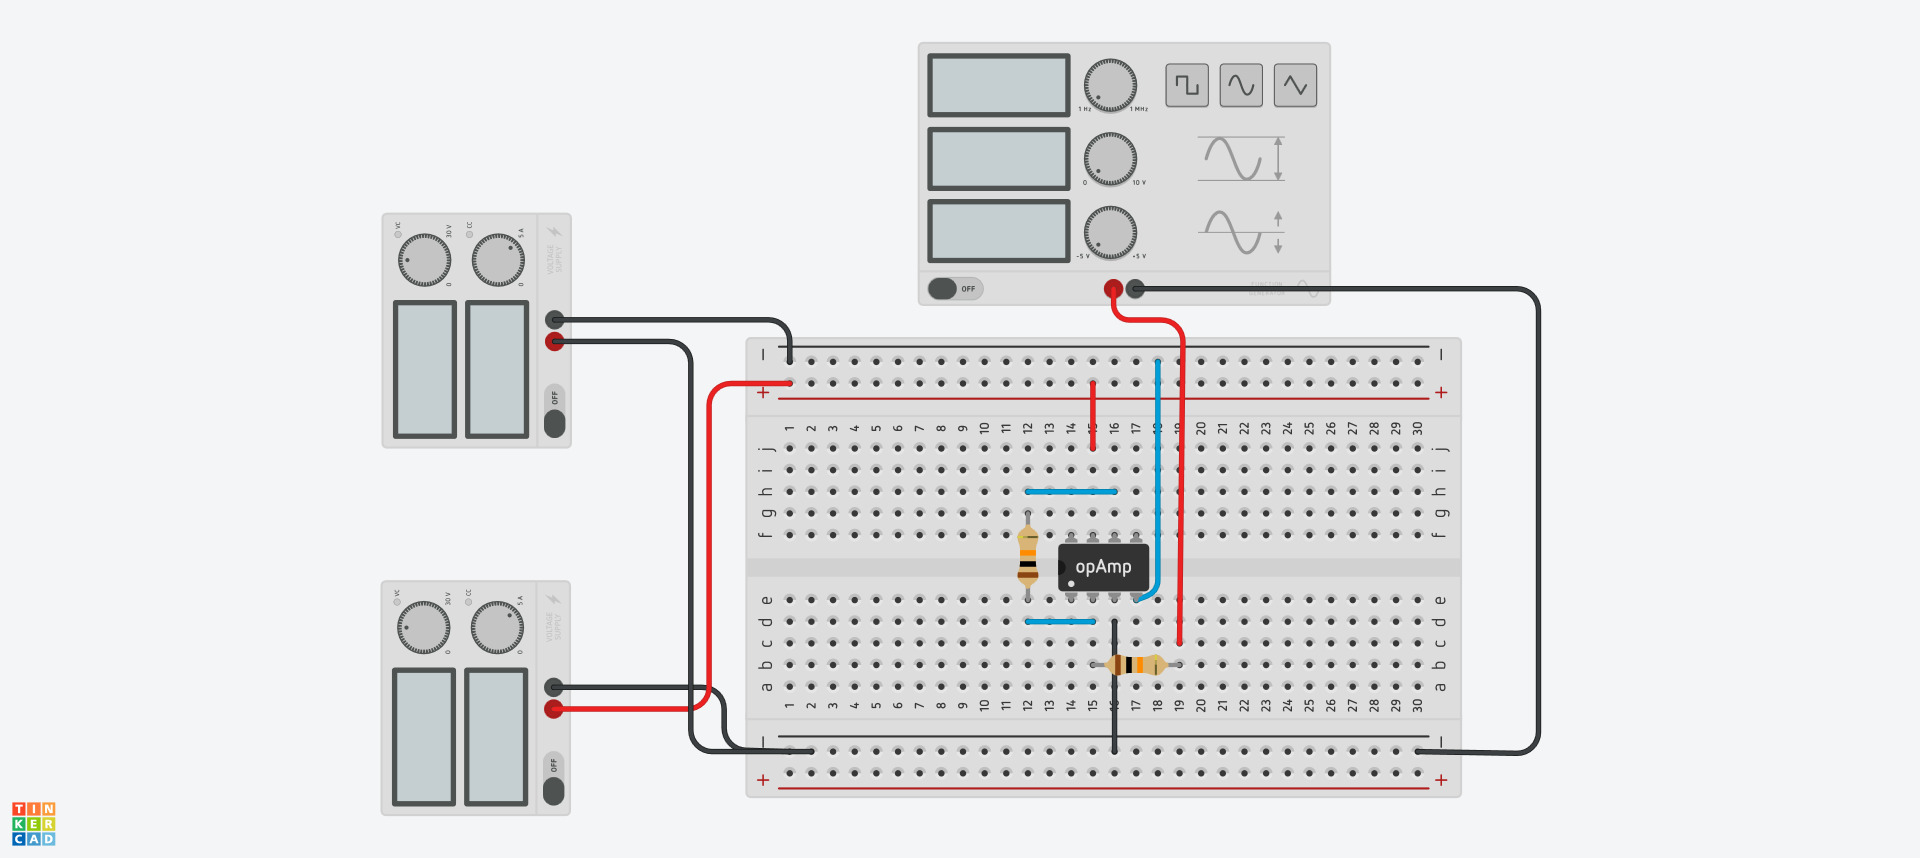
\includegraphics[width=\linewidth]{./res/bread.jpg}
\end{figure}
	
\renewcommand\refname{Βιβλιογραφία}
\printbibliography

\end{document}
